\section{The algorithmic agent}

%%%%%%%%%%%%%%%%%%%%%%%%%%%%%%%%%%%%%%%%%%%%%%%%%%
\begin{frame}[label=ladila]{The algorithmic agent}
Minimal set of elements needed for an interacting homeostatic algorithmic system. %To be connected with (neuro)biology.
 \begin{center}
  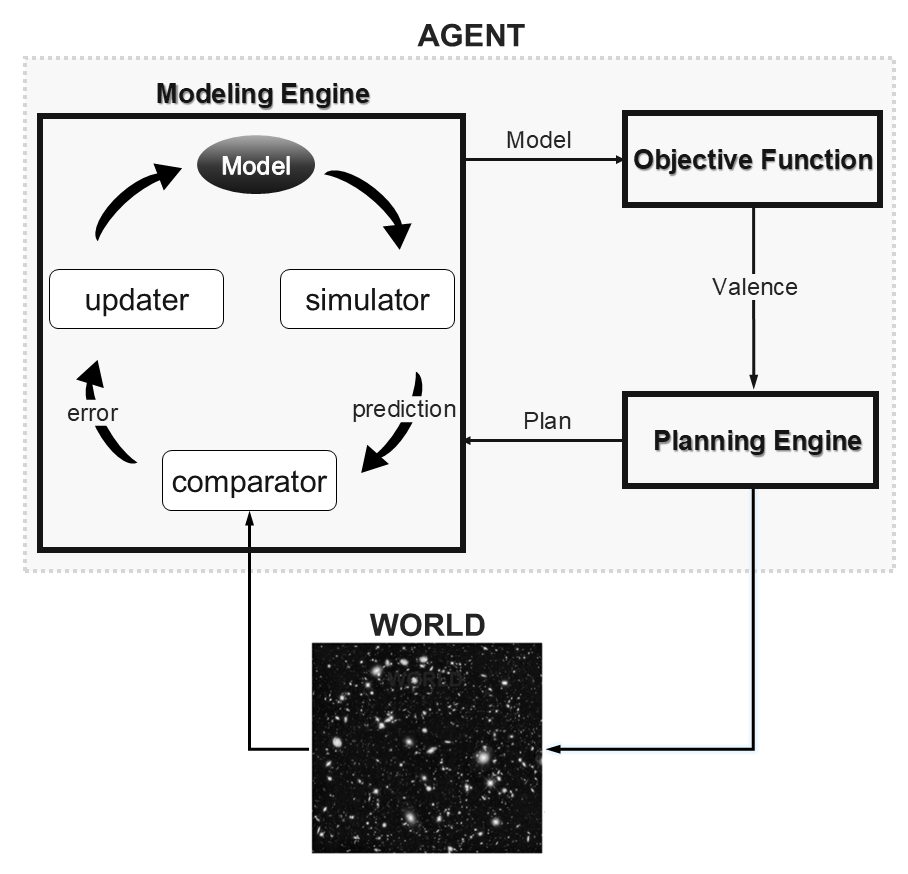
\includegraphics[height=6cm]{img/Figure1_StructuredDynamics.png}
  \end{center}

\end{frame}



%%%%%%%%%%%%%%%%%%%%%%%%%%%%%%%%%%%%%%%%%%%%%%%%%%
\begin{frame}[label=ladila]{The algorithmic event of \SEP}
%Theories of cortical processing emphasize the separation of forward and backward information flow in the cortex also mirrored at the level of single cortical pyramidal cells \citep{CarhartHarris2019,Aru2020}. 

The \textbf{Comparator}, crucial for \SEP, is implemented hierarchically in L5 P cells\citep{CarhartHarris2019,Aru2020} (posterior hot zone). \vspace{0.5cm}

 
  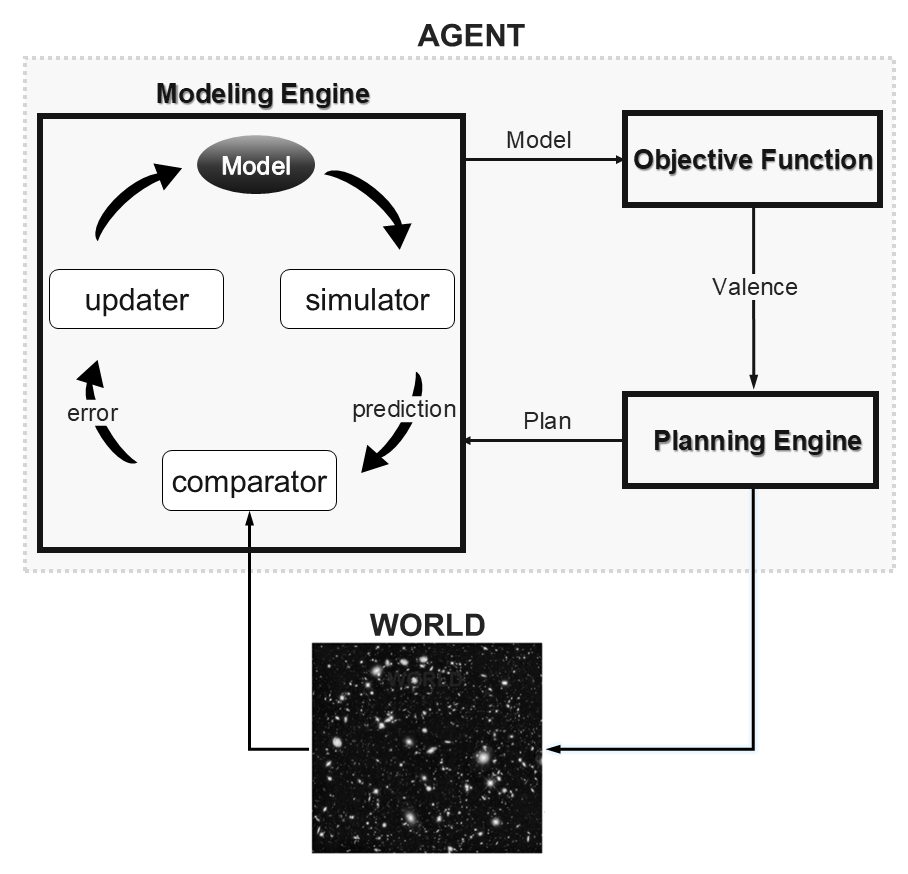
\includegraphics[height=4.cm]{img/Figure1_StructuredDynamics.png}
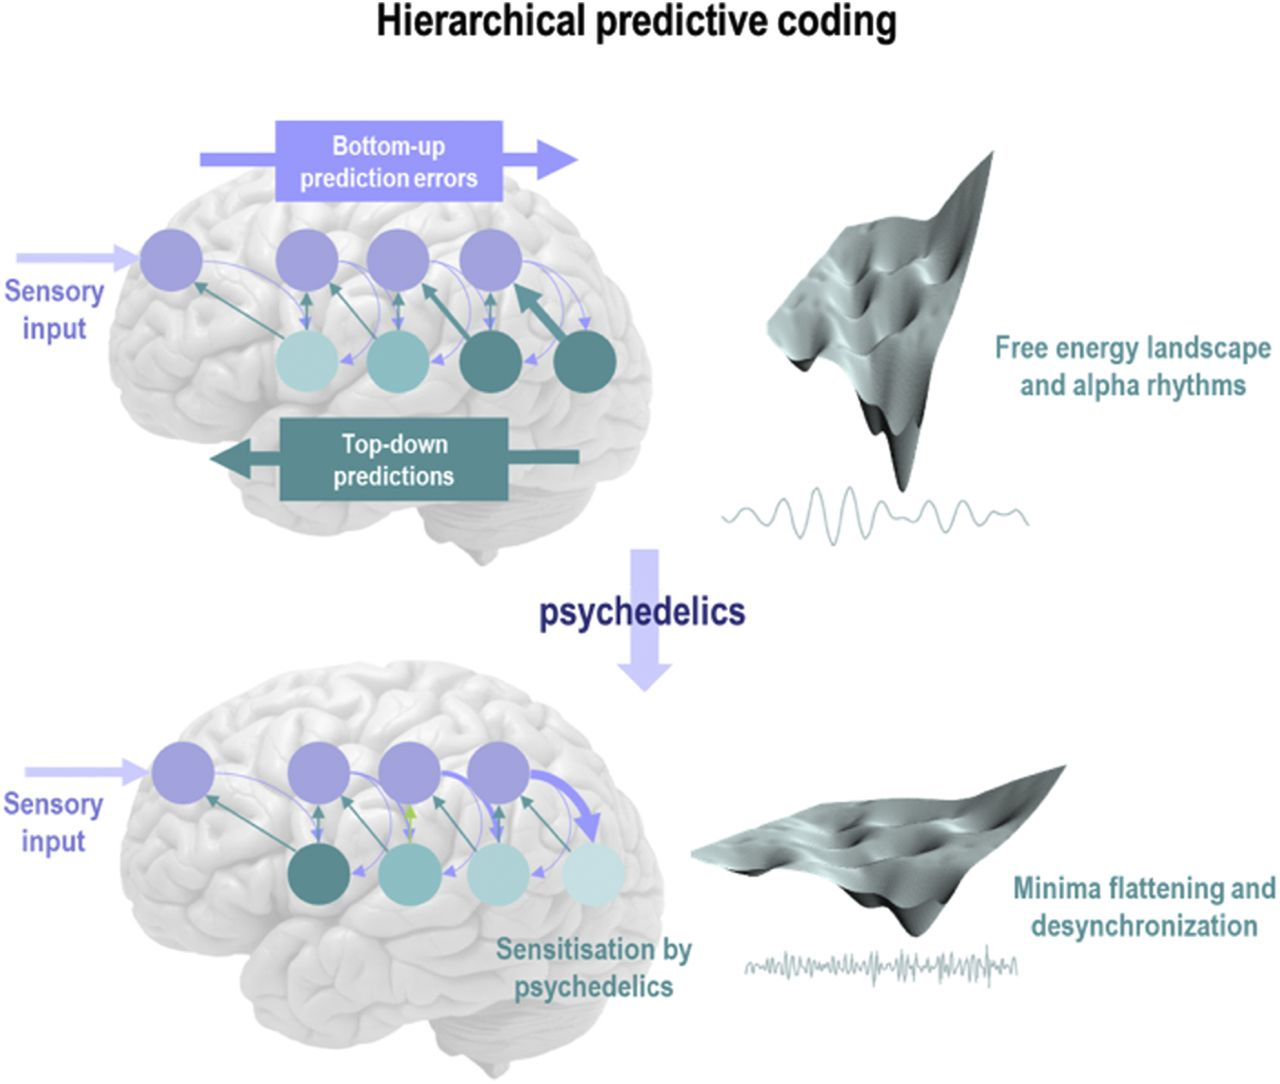
\includegraphics[height=4.cm]{img/F1.large.jpg}
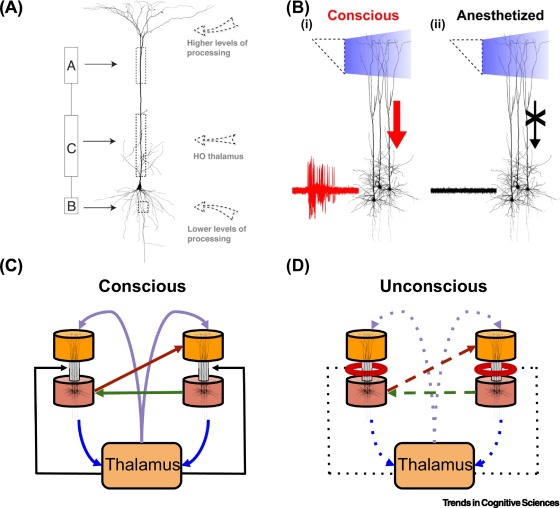
\includegraphics[height=4.cm]{img/gr2.jpeg}
\end{frame}



%%%%%%%%%%%%%%%%%%%%%%%%%%%%%%%%%%%%%%%%%%%%%%%%%%

%%%%%%%%%%%%%%%%%%%%%%%%%%%%%%%%%%%%%%%%%%%%%%%%%%
% \begin{frame}[label=ladila]{Model-building II: intelligence}
%  Evolutive pressure gives rise to the next leap, {\em intelligence}: agents that, starting from their static model (DNA in life)   build higher-level compressive models of the world within their lifetime, e.g., using brains.\vfill
 
%  Importantly, KT holds that both static-model and active-modeling agents enjoy structured experience, only that their level of structure is possibly different.  \vfill
 
 
%  [What comes after life and intelligence?]
 
% \end{frame}


\begin{frame}[label=ladila]{Emotion and Depression \cite{ruffini_algorithmic_2024}}
 
   To include the experience dimension of valence in the agent, we define: 
\begin{definition}[Emotional state or Mood of an Agent] 
The {\bf emotional state} of the Agent is the tuple E = (Model, Valence). 
\end{definition}
In first-person language, {\em emotion is structured experience with valence}, and can be described along dimensions characterizing model structure (simplicity, breadth, accuracy, etc.) plus valence.  
  \begin{definition}[Depressed Agent] 
{\bf Depression} is a pathological state in which the output value of the Objective Function (valence) of an agent is persistently low.
\end{definition}
    
 
\end{frame}
%%%%%%%%%%%%%%%%%%%%%%%%%%%%%%%%%%%%%%%%%%%%%%%%%%
% \begin{frame}[label=ladila]{Model-building in artificial agents}
% As a consequence of the above, we should explore two routes to the construction of artificial model-building agents: \vfill

% A) {\bf Single generation} model building where agents are endowed with a {\em simplicity bias} (this is what we call the  {\em intelligence} approach). \vfill


% B) {\bf Transgenerational} model building ({\em life}) where the bias for simplicity  emerges naturally from the construction process that favors simple short programs  under evolutionary pressure in {\em  environments governed by simple laws}.  
% \end{frame}